\subsection{Einlesen der Konfigurationsdateien}
\paragraph{Klassenstruktur}
Im Hintergrund wird die Klassenstruktur der \acs{gui} nachgebildet. Es gibt eine \enquote{Page}-, eine \enquote{Measurement}- und eine \enquote{Sensor} Klasse. Eine \enquote{Measurement} Instanz kann mehrere \enquote{Sensor} Instanzen enthalten, da manche \enquote{Measurement} zur Berechnung (z.B. der Wärmerückgewinnungsgrad) mehrere Messwerte benötigen. Die \enquote{Page} Instanzen speichern die jeweiligen \enquote{Measurement} Instanzen, die auf dieser Seite angezeigt werden sollen. Die \enquote{Page} Instanzen existieren, damit der ausgelesene Parameter an der richtigen Stelle auf der \acs{gui} verändert werden kann. Es gibt nämlich gleich viele \enquote{Page} Instanzen wie \enquote{PageFrame} Instanzen (vgl. Kapitel \ref{tkintercode}) und gleich viele \enquote{Measurement} Instanzen wie \enquote{MeasurementFrame} Instanzen. (siehe Abb.~\ref{fig:uml_backend}).
\begin{figure}[ht]
	\centering
	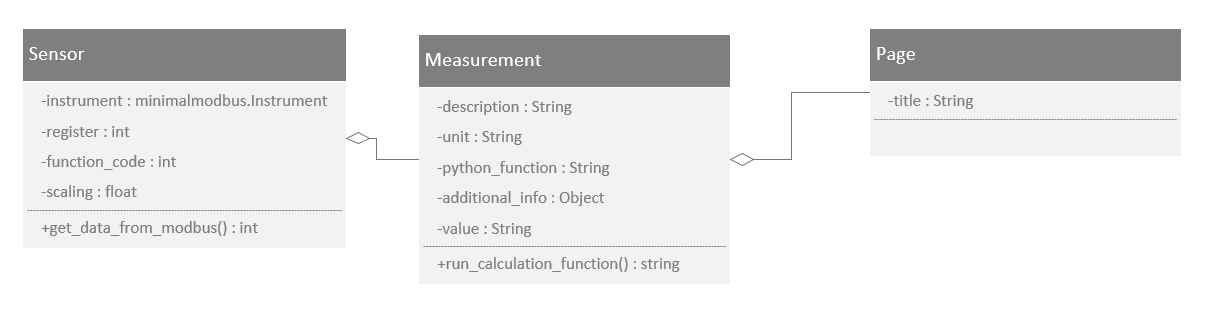
\includegraphics[width=1.0\linewidth]{Bilder/UML_Backend}
	\caption{UML Diagramm Backend}
	\label{fig:uml_backend}
\end{figure}

Die \enquote{Page}-, \enquote{Measurement}- und \enquote{Sensor} Instanzen werden beim Einlesen der Konfigurationsdateien aufgrund der Objekte im \enquote{pages} JSON Arrays (vgl. Kapitel \ref{json_config_files}) erstellt und in Listen gespeichert. \newline
Zum Einlesen werden drei Funktionen implementiert:
\begin{itemize}
	\item \textbf{\enquote{load\_config}:} Diese Funktion lädt die gesamte Haupt-Konfigurationsdatei ein. Es werden die angeschlossenen Geräte ermittelt und die \enquote{Page}-, \enquote{Measurement}- und \enquote{Sensor} Instanzen erstellt. Dafür kommen die beiden folgenden Hilfsfunktionen zum Einsatz.
    \begin{itemize}
		\item \textbf{\enquote{get\_sensor\_unit}:} Liest die Sensor-Konfigurationsdateien ein. Dadurch können den Messwerten die richtigen Maßeinheiten zugewiesen werden.
		\item \textbf{\enquote{get\_sensor\_data}:} Liest aus der Geräte-Konfigurationsdatei am angegebenen Port die Parameter aus und liefert diese Parameter als JSON Objekt zurück. Sie liest das Register, den Modbus Function Code und die Skalierung aus. Die Skalierung wird anhand der Maßeinheit aus der Sensor-Konfigurationsdatei ausgewählt.
	\end{itemize}
\end{itemize}

\paragraph{Einlesen und erstellen der Instanzen}
Einlesen kann man ein JSON Attribut mit folgender Syntax. Im folgenden Beispiel wird aus der Instanz namens \enquote{page} das Attribut title gesucht und zurückgeliefert.
\begin{pythoncode}
title = page["title"]
\end{pythoncode}

In den Codeblöcken wird in den mit \enquote{\#[Inhalt]} gekennzeichneten Zeilen weitere Funktionalität gekennzeichnet, die entweder später beschrieben wird oder zur besseren Übersichtlichkeit ausgelassen werden. 

Im folgenden Code werden die \enquote{Measurement} Instanzen erstellt, indem die anzuzeigenden Messwerte aus dem \enquote{sources} Array iteriert werden. Anhand der Informationen der Objekte im \enquote{sources} Array werden dann die entsprechenden Geräte im \enquote{devices} Array herausgesucht. Es werden weitere Parameter aus der Hauptkonfigurationsdatei ausgelesen, die zu dem entsprechenden Messwert gehören (z.B. die Bezeichnung oder die Einheit). Anschließend werden die \enquote{Sensor} Instanzen erstellt und einer Liste beigefügt, da manche Measurements mehrere Messwerte benötigen. Diese Liste, sowie die vorher ausgelesenen Parameter werden beim Erstellen der \enquote{Measurement} Instanzen dem Konstruktor übergeben und darin in Instanzvariablen gespeichert.
\begin{pythoncode}
page_measurements = []
for measurements in page["sources"]:
	measurements_sensors = []
	#[Auslesen weiterer Parameter der Haupt-Konfigurationsdatei (description, unit, python_function,additional_info)]
	#[Erstellen der Sensor Instanzen (Siehe nächster Codeblock)]
	page_measurements.append(Measurement(description=description, unit=unit, sensors=measurements_sensors, python_function=python_function, additional_info=additional_info))
\end{pythoncode}

Im folgenden Code wird für jeden Port (an jedem Port ist ein \enquote{Sensor} angeschlossen) eines Geräts eine \enquote{Sensor} Instanzen erstellt. Alle \enquote{Sensor} Instanzen werden der \enquote{page\_sensors} Liste beigefügt. Dafür gibt es im \enquote{sources} Array die einzelnen Ports. Das sind Wertepaare, die jeweils aus Gerät und \enquote{Sensor} bestehen (vgl. Kapitel \ref{json_config_files}). Mit diesen beiden Werten kann dann das entsprechende Gerät im \enquote{devices} Array gefunden werden und darin der entsprechende Port im \enquote{sensors} Array. Mit der \enquote{get\_sensor\_unit} Funktion wird die Einheit erhalten und mit der \enquote{get\_sensor\_data} Funktion weitere Sensordaten. Diese werden beim Erstellen der \enquote{Sensor} Instanz dem Konstruktor übergeben.
\begin{pythoncode}
port_counter = 0
for port in port_arr:
	device_id = list(port.keys())[port_counter] # example: QBM1
	port_id = port[device_id]  # example: AI1
	port_counter += 1
	
	for device in config_full_data[0]["devices"]:
		if device["id"] == device_id:
			#[Aufruf der get_sensor_unit Funktion]
			#[Auslesen der Geräteparameter in der Haupt-Konfigurationsdatei (baud_rate, mbaddress etc.)]
			#[Aufruf der get_sensor_data Funktion]
			measurements_sensors.append(Sensor(baud_rate=device["baud_rate"], ..., register=register, zero_based=device["zero_based"]))
\end{pythoncode}

Die \enquote{Measurement} Instanzen sind nach dem Erstellen alle in einer Liste gespeichert. Zum Schluss werden \enquote{Page} Instanzen erstellt. Die \enquote{Measurement} Liste wird so aufgeteilt, dass maximal 5 Measurements auf einer Seite sind. Anhand dieser \enquote{Page}- und \enquote{Measurement} Instanzen wird beim Erstellen der \acs{gui} die Anzahl an Seiten übernommen, der Seitentitel und die Beschreibungen der Messwerte gesetzt (siehe Kapitel \ref{gui_design}). 
\begin{pythoncode}
counter = 0
last_slice = 0
for measurement in page_measurements:
	counter += 1
	if ((counter % 5) == 0) or (counter == len(page_measurements)):
		all_pages.append(Page(title=title, measurements=page_measurements[last_slice:counter]))
		last_slice = counter
\end{pythoncode}

%\pythonfile[firstline=125, lastline=197]{Code/modbus.py}

Im Konstruktor der \enquote{Page}- \enquote{Measurement}- und \enquote{Sensor} Klasse werden die ausgelesenen Variablen in Instanzvariablen gespeichert.